\section{Prior Models}\label{foi.prior}
The earliest HIV transmission models \cite{Anderson1986}
were adapted from models of other sexually transmitted diseases,
especially gonorrhea \cite{Yorke1978,Nold1980,Hethcote1982}.
These early HIV transmission models did not explicitly model individual sex acts,
but instead assumed an overall probability of transmission per partnership \cite{Isham1988}.
This assumption was initially justified via data suggesting that
the probability of HIV transmission per partnership
increased quickly and then saturated \cite{Kaplan1990}.
Such data were later explained by heterogeneity in
infectiousness (\eg due to infection stage, etc.) and/or
susceptibility (\eg due to genital ulcer disease, etc.)
\cite{Gray2001,Rottingen2002,Boily2009}.
As this heterogeneity was quantified \cite{Gray2001}
and incorporated into HIV transmission models \cite{Moghadas2003},
the probability of transmission was increasingly parameterized per act \vs per partnership.
% TODO: cite?
\par
The shift to per-act \vs per-partnership parameterization highlighted
a fundamental limitation of compartmental models
(including pair-based models, see \sref{foi.prior.lims}):
compartmental models cannot model individual partnerships,
because each ``compartment'' reflects a group of individuals
whose characteristics are assumed to be homogeneous \cite{Rao2021}.
Therefore, the dynamics of sexual partnerships must be modelled using
average rates of partnership change and average characteristics of those partnerships.
As a result, partnerships are effectively modelled as instantaneous, such that
the cumulative risk of transmission per partnership
is applied at the moment of partnership change \cite{Dietz1988a}.
This cumulative risk can be defined in terms of
the average total numbers of sex acts per partnership,
but the timing of specific sex acts or other events within partnerships
cannot be captured in compartmental models.
Further implications of the ``instantaneous partnership assumption''
and alternate modelling frameworks which avoid this assumption
are discussed in \sref{foi.prior.lims} and \sref{foi.prop}.
\par
Thus, over the years, different force of infection equations
have been designed for compartmental models which
explicitly aggregate the risk of transmission across different numbers and types of sex acts,
and likewise across different numbers and types of sexual partners/partnerships.
The remainder of this section reviews these equations and their assumptions in detail.
% ==================================================================================================
\subsection{Aggregating Sex Acts within a Partnership}\label{foi.prior.bhom}
To account for repeated sex acts with the same partner,
the per-partnership probability of transmission $B$ was conceptualized as follows. % TODO: cite?
Let $A$ denote the total number of sex acts in the partnership,
and $\beta$ denote the probability of transmission per act.
For now, $\beta$ is assumed to be equal for all acts.
With equal and independent $\beta$,
the theoretical probability of $n$ transmissions after $A$ acts
can be described by a binomial distribution:
\begin{equation}\label{eq:B.n}
  p(n) = {A \choose n}\,\beta^n\,{(1 - \beta)}^{A-n}
\end{equation}
Since transmission of HIV can actually only occur once,
the per-partnership probability of transmission $B$ is defined via
the probability of ``escaping'' infection after all $A$ acts:%
\footnote{\eqref{eq:B} can also be reasonably approximated
  via the Poisson distribution $B = 1 - e^{-\beta A}$ for small $\beta$.}
\begin{alignat}{1}\label{eq:B}
  B &= 1 - p(n = 0) \nonumber\\
  &= 1 - {A \choose 0}\,\beta^0\,{(1 - \beta)}^{A} \nonumber\\
  &= 1 - {(1 - \beta)}^A
\end{alignat}
We can show that $B \le \beta A$.
Thus, a model with partnerships using \eqref{eq:B}
reduces transmission \vs a model without partnerships
by adjusting for ``wasted contacts''.
Figure~\ref{fig:binom.dur} illustrates the shape of $B(A)$ (curve)
and the corresponding effective probabilities of transmission per act $B/A$ (tangent slopes)
for a shorter (red) \vs longer (blue) partnership.
Although $B(A)$ is monotonic, the effective probability of transmission per act
decreases with the number of acts because, on average,
more and more acts are ``wasted'' --- occuring after transmission.
% The average proportion of post-transmission acts (PTA)
% also increases with the per-act probability of transmission $\beta$, according to:
% \begin{equation}\label{eq:pte}
%   P_{PTA} = 1 - \frac{B(A)}{\beta A}
% \end{equation}
\begin{figure}
  \centerline{
  \begin{subfigure}[b]{.5\linewidth}
    \centering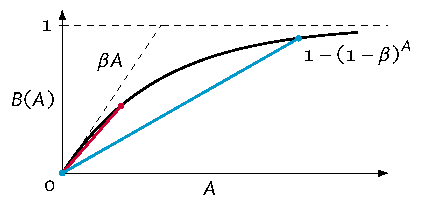
\includegraphics[scale=1]{binom.dur.pdf}
    \caption{Probability of transmission per partnership $B$ \vs number of sex acts $A$,
      comparing shorter (red) \vs longer (blue) partnerships}
    \label{fig:binom.dur}
  \end{subfigure}\quad%
  \begin{subfigure}[b]{.5\linewidth}
    \centering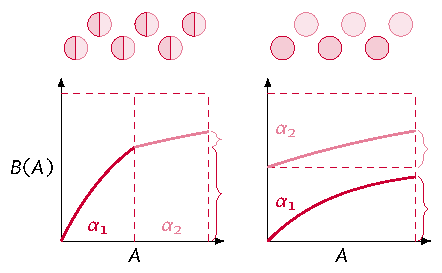
\includegraphics[scale=1]{binom.dots.xph.pdf}
    \caption{Average accumulation of transmission probability for
      within-partnership heterogeneity (red) \vs
      between-partnership heterogeneity (blue)}
    \label{fig:binom.xph}
  \end{subfigure}}
  \caption{Per-partnership robability of transmission \vs number of acts}
  \label{fig:binom}
  \floatfoot{
    $B$: probability of transmission per partnership;
    $\beta$: probability of transmission per act;
    $A$: total acts per partnership;
    $\alpha$: fraction of total acts (within or between partnerships).}
\end{figure}
% ==================================================================================================
\subsection{Heterogeneity in the Per-Act Probability of Transmission}\label{foi.prior.bhet}
As noted above, the per-act probability of transmission $\beta$ is heterogeneous,
varying with factors like: HIV infection stage, genital ulcer disease, condom use, etc.
\cite{Boily2009,Giannou2016}.
The next step in developing a force of infection equation is to extend \eqref{eq:B}
to allow heterogeneity in $\beta$.
Let $\beta_f$ denote the probability of transmission associated
with a particular factor (or combination of factors) $f$; and
let $\alpha_f$ denote the proportion of acts $A$ in an average partnership
having transmission probability $\beta_f$
(thus $\Sigma_f \alpha_f = 1$).
There are two approaches to aggregating $\beta_f$,
reflecting different interpretations of $\alpha_f$:%
\footnote{In most compartmental models without repeated contacts (partnerships),
  this distinction is not possible or necessary, because
  all contacts (sex acts) between two compartments (risk groups) are assumed to be independent.}
\pagebreak % TEMP
\begin{itemize}
  \item \textbf{{Within}-Partnership Heterogeneity (WPH)}:
  modelled partnerships are identical, but comprise heterogeneous acts
  --- $\alpha_f$ denotes a proportion of acts in each partnership
  (Figure~\ref{fig:binom.xph} red).
  % \emph{some acts in all partnerships}
  \begin{equation}\label{eq:B.wph}
    B_{\wph} = 1 - \prod_f {(1 - \beta_f)}^{A\alpha_f}
  \end{equation}
  \item \textbf{{Between}-Partnership Heterogeneity (BPH)}:
  modelled partnerships are different, but each comprise identical acts
  --- $\alpha_f$ denotes a proportion of partnerships
  (Figure~\ref{fig:binom.xph} blue).
  % \emph{all acts in some partnerships}
  \begin{equation}\label{eq:B.bph}
    B_{\bph} = 1 - \sum_f \alpha_f {(1 - \beta_f)}^{A}
  \end{equation}
\end{itemize}
Figure~\ref{fig:binom.xph} illustrates these approaches for a simple case with two factors.
For WPH (red), each factor $f$ marginally contributes to
the probability of escaping infection in every partnership.
For BPH (blue), the overall probability of escaping infection is modelled as
a weighted average across partnerships, each affected by a single factor $f$.
Both approaches guarantee $B < 1$,
but we can show that $B_{\wph} \ge B_{\bph}$
by the (weighted) AM-GM inequality (see \sref{app.math.misc.xph}) \cite{Aldaz2009}.
% TODO: discuss how these two options are used willy-nilly
Intuitively, this inequality arises because
any large probability of transmission $\beta_f$
has disproportionate influence in \eqref{eq:B.wph},
even for a small proportion of acts affected $\alpha_f$,
whereas this influence is bounded by $\alpha_f$ in \eqref{eq:B.bph},
as shown in Figure~\ref{fig:binom.xph}.
\par
% \eqref{eq:B.wph} appears to be a ``natural'' extension of \eqref{eq:B},
% but the interpretation should be considered carefully.
The decision to use WPH \vs BPH for aggregating specific types of heterogeneity in $\beta$
should be driven by the factor(s) in question.
To this end, it is possible to combine \eqref{eq:B.wph} and \eqref{eq:B.bph} as follows
to aggregate both types of factors simultaneously:
\begin{equation}\label{eq:B.xph}
  B_{wb} = 1 - \sum_g \gamma_g \prod_f {(1 - \beta_{fg})}^{A\alpha_{fg}}
\end{equation}
where:
$f$ denotes WPH factor(s);
$g$ denotes BPH factor(s); and
$\gamma_g$ replaces $\alpha_f$ for BPH factors.
Then, for example, if it is known or assumed that
``50\% condom use'' reflects 50\% condom use in 100\% of partnerships,
sex acts with condoms \vs without condoms
should be aggregated as WPH, with $\alpha_f = 0.5$.
By contrast, heterogeneity in individual-level factors like infection stage or treatment status
should be aggregated as BPH,%
\footnote{Individual-level factors should be aggregated as BPH because
  a given partner has exactly one current infection stage or treatment status;
  of course, this stage/status could evolve over the course the partnership,
  but this future trajectory is not explicitly modelled
  --- which only serves to highlight the limitations of
  either approach to aggregating heterogeneity in $\beta$.}
with $\gamma_g$ as the conditional prevalence of each stage/status~$g$ among infected partners.
In fact, aggregating infection stage and treatment status
is often deferred to the full incidence equation (\sref{TODO}) using an equivalent form,
but where $\gamma_g$ is replaced by
the unconditional prevalence of stage/status~$g$ among \emph{all} partners.
% TODO: anything else to add?
% ==================================================================================================
\subsection{Aggregating Partnerships}\label{foi.prior.part}
Although we considered between-partnership heterogeneity in \sref{foi.prior.bhet},
the modelled per-partnership probability of transmission $B$
still corresponds to a single average partnership.
Some population groups may have multiple partners per unit time (usually year),
possibly including different types of partnerships,
or indeed less than one partnership per year, on average.
Thus, the second step in constructing the incidence equation is to
aggregate transmission risk across these various partnerships.
\par
As in \sref{foi.prior.bhet}, there are two main approaches to aggregating partnerships
--- indeed having similar equations to Eqs.~(\ref{eq:B.wph})~and~(\ref{eq:B.bph}).
This time, the distinction is familiar:
\begin{itemize}
  \item \textbf{Incidence Rate:}
  instantaneous rate of infection among susceptible individuals
  --- transmission risks are addative; can have $\lambda_i > 1$.
  \begin{equation}\label{eq:foi.ir}
    \lambda_i^\ir = \sum_{ki'h'} Q_{kii'} B_{kii'h'} \frac{{I}_{i'h'}}{N_{i'}}
  \end{equation}
  \item \textbf{Incidence Proportion:}
  cumulative proportion of susceptible individuals infected over a period $\Delta_t$
  --- transmission risks are competing; can only have $\lambda_i \le 1$.%
  % TODO issue of different time periods modelled in B ?
  \footnote{If all transmission modifiers $f$ are modelled as WPH via \eqref{eq:B.wph},
    then \eqref{eq:foi.ip} could further simplify to effectively model
    all sex acts across all partnerships during the period $\Delta_t$
    as competing risks --- \ie in the exponent: $Q_{kii'} A_k \alpha_{kf} \Delta_t$.}
  \begin{equation}\label{eq:foi.ip}
    \lambda_i^\ip = 1 - \prod_{ki'h'} \frac{{I}_{i'h'}}{N_{i'}} {(1 - B_{kii'h'})}^{Q_{kii'} \Delta_t}
  \end{equation}
\end{itemize}
where:
$Q_{kii'}$ is the rate of type-$k$ partnership formation between groups $i$ and $i'$,%
\footnote{This partnership formation rate $Q_{kii'}$ is often broken down into
  a partnership formation rate $Q_{ki}$ and a mixing matrix $\rho_{pii'}$,
  as in \sref{model.par.mix.eps}.}
% --- distinguished from the more generic ``contact rate'' $C_{kii'}$ from \eqref{eq:foi.strat},
$B_{kii'h'}$ is the average per-partnership probability of transmission
from group/infection stage $i'h'$ to group $i'$ via partnership type $k$,
and $I_{i'h'}/N_{i'}$ is the prevalence of infection stage $h'$ among group $i'$.
\par
By definition, the force of infection is a rate \cite{Anderson1991}.
Yet in principle, incidence proportion could be more precise than incidence rate
\emph{over a given time period $\Delta_t$}.
Since most models are now solved computationally,
the period $\Delta_t$ could be matched to the timestep of the numerical solver.
However, the added precision may be insignificant, as $\Delta_t$ should be small.%
\footnote{Also, many popular numerical solvers do not pass the timestep $\Delta_t$
  (only the current time $t$) to the derivative computing function,
  and may use adaptive timestep sizes for precision while solving --- including:
  \href{https://docs.scipy.org/doc/scipy/reference/generated/scipy.integrate.odeint.html}
  {\texttt{scipy.integrate.odeint}} in Python,
  \href{https://cran.r-project.org/web/packages/deSolve/index.html}
  {\texttt{deSolve::lsoda}} in R, and
  \href{https://www.mathworks.com/help/matlab/ref/ode45.html}
  {\texttt{ode45}} in MATLAB.}
Moreover, some applications of this approach have used
a period of $\Delta_t = 1$ year in the equation, but then
applied the resulting incidence proportion $\lambda_i^\ip$ as a rate over smaller timesteps.
Such applications then erroneously reduce \emph{current} transmission
due to \emph{future} ``wasted contacts'' across multiple partnerships.
This reduction is then redundant because
``wasted contacts'' \emph{within} partnerships are already captured via
the per-partnership probability of transmission, while
``wasted contacts'' \emph{between} partnerships are already captured via
multiple opportunities for transmission over successive timesteps.
In sum, unless the period $\Delta_t$ can be matched to the numerical solver timestep,
incidence rate \eqref{eq:foi.ir} is preferred over incidence proportion \eqref{eq:foi.ip}
as the force of infection equation.
% cite Diekmann2021 ?
% ==================================================================================================
\subsection{Revisiting Partnership Duration}\label{foi.prior.dur}
A final issue in constructing the force of infection equation relates to parameterization.
In Eqs.~(\ref{eq:B.n})--(\ref{eq:foi.ip}),
partnership durations $\delta$ are not explicitly modelled,
but implied by the total numbers of sex acts per partnership $A$,
and a presumed frequency of sex per partnership $F$, such that $A = F\delta$.
By contrast, the partnership formation rate $Q$ is often directly informed by survey questions like
\shortquote{How many different people have you had sex with in the past 12 months?}
As such, the lowest possible value among sexually active individuals
would appear to be $Q = 1$ (per year).
Then, if $Q \ge 1$ is used in the model,
the total sex acts per partnership are (and should be) reduced to reflect up to one year
--- \ie $A \le F$, or effectively $\delta \le 1$ year.
This change \vs $Q < 1, A > F$
can substantially reduce the proportions of sex acts which are modelled as ``wasted'',
and thus increases transmission via longer ($\delta > 1$ year) partnerships.
On the other hand, using the true $Q < 1, A > F$
can effectively delay early transmission in longer partnerships,
such that modelled HIV prevalence could lag behind true HIV prevalence.
These dynamics are further explored in \sref{foi.exp.model}.
\par
Lastly, it is worth noting that partnership duration $\delta$ is further related to
the average partnership formation rate $Q$ and
the average number of concurrent partners $K$ by $Q = K/\delta$.%
\footnote{Gaps between partnerships do not result in $Q < K/\delta$,
  because the average $K$ would be reduced if some individuals are ``between partnerships''.}
Thus, an alternate parameterization might specify
the number of concurrent partners $K$ and the frequency of sex with each partner $F$.
The overall rate of sex would be the same: $QA = KF$.
In some ways, this $KF$ parameterization is more intuitive,
and it will be useful later, in the new force of infection approach (\sref{foi.prop}).
% ==================================================================================================
\subsection{Limitations and Alternate Modelling Frameworks}\label{foi.prior.lims}
TODO